\documentclass[xcolor={dvipsnames}]{beamer}
\usepackage[utf8]{inputenc}
\usepackage[english, russian]{babel}

\usetheme{Madrid}
\usecolortheme{default}
\setbeamertemplate{enumerate items}[default]
\setbeamercolor*{structure}{bg=white,fg=black}

% \setbeamercolor*{palette primary}{use=structure,fg=white,bg=structure.fg}
% \setbeamercolor*{palette secondary}{use=structure,fg=white,bg=structure.fg!75}
% \setbeamercolor*{palette tertiary}{use=structure,fg=white,bg=structure.fg!50!black}
% \setbeamercolor*{palette quaternary}{fg=white,bg=black}

% \setbeamercolor{section in toc}{fg=black,bg=white}
% \setbeamercolor{alerted text}{use=structure,fg=structure.fg!50!black!80!black}
% \setbeamercolor{frametitle}{bg=black,fg=white}

% \setbeamercolor{titlelike}{parent=palette primary,fg=structure.fg!50!black}
% \setbeamercolor{frametitle}{bg=gray!10!white,fg=black}

% \setbeamercolor*{titlelike}{parent=palette primary}

% \setbeamercolor{block title example}{bg=black,fg=white}

% \usepackage{times,url}

% \setbeamertemplate{footline}[frame number]
% \setbeamertemplate{footline}[frame number]{}

\setbeamertemplate{footline}{}

\setbeamertemplate{footline}
% {
%   \leavevmode%
%   \hbox{%
%   \begin{beamercolorbox}[wd=.333333\paperwidth,ht=2.25ex,dp=1ex,center]{author in head/foot}%
%     \usebeamerfont{author in head/foot}\insertsection
%   \end{beamercolorbox}%
%   \begin{beamercolorbox}[wd=.333333\paperwidth,ht=2.25ex,dp=1ex,center]{title in head/foot}%
%     \usebeamerfont{title in head/foot}\insertsubsection
%   \end{beamercolorbox}%
%   \begin{beamercolorbox}[wd=.333333\paperwidth,ht=2.25ex,dp=1ex,right]{date in head/foot}%
%     \usebeamerfont{date in head/foot}\insertshortdate{}\hspace*{2em}
%     \insertframenumber{} / \inserttotalframenumber\hspace*{2ex} 
%   \end{beamercolorbox}}%
%   \vskip0pt%
% }

%------------------------------------------------------------
%This block of code defines the information to appear in the
%Title page
\title[ALBERT for SQuAD 2.0] %optional
{ALBERT for Question Answering on SQuAD 2.0}

% \subtitle{A short story}

\author[Тохчуков Данил] % (optional)
{Тохчуков Данил}

\institute[Institute] % (optional)
{
    Факультет вычислительной математики и кибернетики\\
    МГУ имени М. В. Ломоносова
}

\date[Article 2023] % (optional)
{2023}

% 右下角使用logo的方式
% \logo{\includegraphics[height=1cm]{overleaf-logo}} 

%End of title page configuration block
%------------------------------------------------------------



%------------------------------------------------------------
%The next block of commands puts the table of contents at the 
%beginning of each section and highlights the current section:

\AtBeginSection[]
{
  \begin{frame}
    \frametitle{Table of Contents}
    \tableofcontents[currentsection]
  \end{frame}
}
%------------------------------------------------------------


\begin{document}

%The next statement creates the title page.
\frame{\titlepage}



\begin{frame}
\frametitle{Введение}

\begin{center}
    Вопросно-ответные системы используются для того, чтобы помочь людям эффективно находить релевантную информацию.
    В статье решается задача Question Answering на датасете SQuAD 2.0.
    Среди существующих вопросно-ответных систем рассматриваются SOTA системы на основе предобученного трансформера ALBERT, и вопросно-ответная система Bidirectional Attention Flow (BIDAF). Также предлагается собственная вопросно-ответная система на базе ALBERT и Bidirectional Attention Flow (BIDAF). Система сохраняет логику BIDAF и использует идеи из SOTA систем на базе ALBERT.
\end{center}

\end{frame}

\begin{frame}
\frametitle{Данные}

\begin{figure}[!ht]
    \centering
    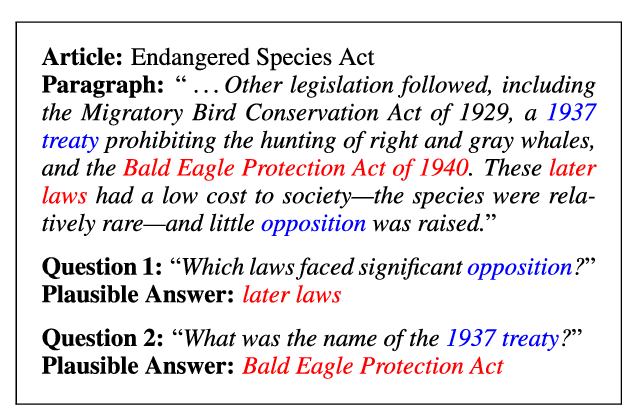
\includegraphics[width=80mm]{../figures/squad_example.png}
    % \caption{Пример из SQuAD 2.0}
    % \label{fig:squad}
\end{figure}

Датасет SQuAD 2.0 состоит из 130,319 объектов обучающей выборки и 11,873 объектов тестовой выборки. В обучающей выборке 33\% объектов не имеют ответа на вопрос, в валидационной же 50\% объектов без ответа.

\end{frame}

\begin{frame}
\frametitle{Постановка задачи}
Задача состоит в том, чтобы найти правильный ответ на заданный вопрос по тексту, причём ответ на
вопрос непрерывен и целиком находится в тексте –- это значит что он не разделяется другими токенами
из текста. Требуется найти начало и конец ответа -- задача классификации.

Если в тексте не будет искомого ответа, модель должна вывести что ответа нет.

\end{frame}

\begin{frame}
\frametitle{Метрики}
Для измерения качества моделей применяются две метрики: Exact Match (EM) score и F1
score.

\textbf{Exact Match} это двоичная мера (истина/ложь) того, точно ли выходные данные системы соответствуют
основному истинному ответу (exact match accuracy). Это довольно строгий показатель.

\textbf{F1} менее строгая метрика. Она является средним гармоническим precision и recall модели. \\
$$F1 = 2*\frac{\text{precision}*\text{recall}}{\text{precision} + \text{recall}}$$
\end{frame}

\begin{frame}
\frametitle{Существующие системы}
\textbf{A Lite BERT(ALBERT)} -- языковая модель с механизмом Self-Attention. На основе ALBERT строилась SOTA вопросно-ответная система ALBERT (ensemble):

\begin{figure}[!ht]
    \centering
    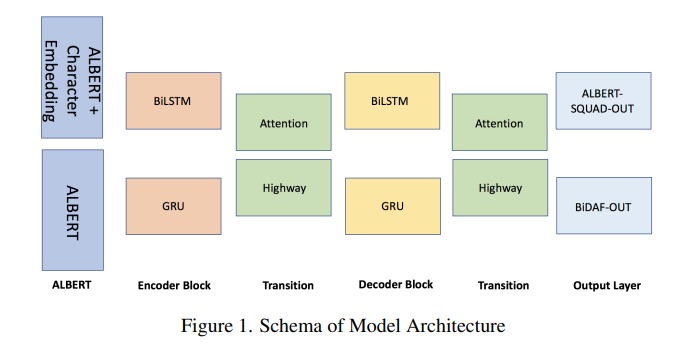
\includegraphics[width=50mm]{../figures/ALBERTsquad.png}
\end{figure}

\textbf{BIDAF} -- полноценная вопросно-ответная система, успешно применявшаяся к задача Question Answering на датасете SQuAD 1.0.
\end{frame}

\begin{frame}
\frametitle{Предложенная система}
\begin{figure}[!ht]
    \centering
    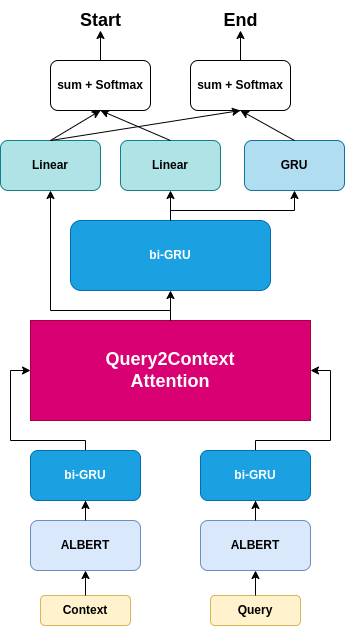
\includegraphics[width=40mm]{../figures/model_diagram.drawio.png}
\end{figure}
\end{frame}

\begin{frame}
\frametitle{Заключение}
В работе была решена задача Question Answering на датасете SQuAD 2.0. Также в работе были представлены основные существующие системы для решения Question Answering задачи. Также была предложена архитектура "облегченной" вопросно-ответной системы на базе языковой модели ALBERT.
\end{frame}

\end{document}
